\documentclass{article}
\usepackage{graphicx} % Required for inserting images
\graphicspath{ {figures/} }
\usepackage{array}
\usepackage{float}
\usepackage{caption}
\usepackage{amsmath}
\usepackage{amsfonts}
\newcommand{\C}{{\mathbb C}}
\newcommand{\E}{{\mathbb E}}
\newcommand{\R}{{\mathbb R}}
\newcommand{\Prr}{{\mathbb P}}
\newcommand{\N}{{\mathbb N}}
\newcommand{\D}{{\mathbb D}}
\newcommand{\Z}{{\mathbb Z}}
\usepackage{hyperref}
\usepackage{pgfplotstable}
\usepackage{booktabs}
\usepackage{array}
\usepackage{colortbl}

% Redefine the format for figure captions
\captionsetup[figure]{
    labelfont={bf},   % Make the label bold (e.g., "Figure 1")
    labelsep=colon,   % Set the separator after the label (optional, default is a colon)
}


\title{Multiperiod Collection of Results}
\author{Prof. Serhiy Kozak \& James Zhang}
\date{\today}

\begin{document}

\maketitle

\tableofcontents

\newpage

\section*{Updates}
\begin{itemize}
    \item Small things like annualizing of Sharpe ratios in graphs, removing industry and constant factors in datasets
    \item Implemented formulas in the paper for mean and covariance matrix of basis assets in our primary tensor approach, results significantly improved
    \item Implemented benchmark models (precise tensor approach, pooled PCA approach, multiperiod (aggregate) PCA)
    \item Incorporating daily data into this framework proved a little bit cumbersome $\implies$ did not 
    provide much more performance improvement.
    \item To-Do: a plausible explanation is due to the data imputation, which could help uncover patterns in the data. Specifically, these patterns may be driven by stocks with missing observations, perhaps because market participants trading these strategies
    only arbitraged away mispricing in stocks for which data was readily available. We should investigate this further at some point. TL;DR - results for OOS Characteristic Anomalies are unsatisfactory, 
    and overall, Full-Sample + OOS PooledPCA and OOS Multiperiod PCA WRDS results are interesting, how much imputation here?
    \item To-Do: experiment with the mean-variance procedure (SCS, RP-PCA) as right now we are currently using the Markowitz formula with $0$ regularization
    \item To-Do: implement T-FF6 and compare to FF6?
\end{itemize}

\section{Setup}

All $R$ tensors are \emph{log} returns, not simple and not excess of the one-lag return \footnote{Clarify that returns are excess of the risk-free rate, they should be, I know it is for the Characteristics Anomalies dataset}. 
The out-of-sample period for all datasets is 
post January 2005. \footnote{We should standardize this to be 01-31-2005 to 2020-08-01, but in the preliminary, should not be a huge difference across 
the datasets.} In our primary specification, 

\begin{itemize}
    \item Rolling window size $W$ is fixed at $120$ months.
    \item Maximum horizon $S$ is fixed at $36$ months.
    \item Maximum lag (lagged characteristics) is $36$ months.
    \item For each dataset and setting, we experiment with $K = 1, 3, 5, 10, 15, 20, 25$, where 
    $K$ represents the rank of PARAFAC and PCA ie. the number of factors.
extracted from the tensor or matrix, respectively. 
    \item Default $\gamma = 0$, we do not yet experiment with RP-PCA in the MVE procedure.
\end{itemize}

For robustness purposes, we present multiperiod results for each of the following $3$ datasets:

\begin{enumerate}
\item Characteristics Anomalies dataset: 1972-06-01 (ie. $\min(t - L)$)  to 2020-08-01
.
- $43$ characteristic-sorted portfolios (SortedFactors)

\item SCS dataset: 1972-07-31 to 2021-12-31

- $44$ characteristic-based portfolios (UnivariateFactors). All industry and constant factors are now removed.

\item WRDS dataset: 1975-01-31 to 2020-12-31

- $107$ characteristic-based portfolios (UnivariateFactors). I believe this dataset still currently has imputed data points, so we should get a version of this with $0$ imputed data points.


\end{enumerate}

For the Characteristic Anomalies dataset, factors are decile-sorted long-short portfolios. For the SCS and WRDS datasets, 
each stock is weighted by its characteristic signal value
and signals are based on cross-sectional ranks, centered and normalized. 


\section{Models}

\subsection{Tensor Factor Model (Approximate)} \label{approx}

This is the primary model outlined in the paper. For time $T$ and horizon $S$, slice the window of three-dimensional data $R \in \R^{W \times L \times N}$, apply PARAFAC to obtain 
\[R_{t, i, l} = \sum_{k=1}^K \lambda_k F_{t, k} B_{t, k} W_{l, k}\]
or in tensor notation
\begin{align}
    R = \sum_{k=1}^K \lambda_k \cdot F \circ B_k \circ W_k \ \ \ \text{ for } F \in \R^{T \times K}, B \in \R^{N \times K}, W \in \R^{L \times K} \label{parafac}
\end{align}
For clarity, let us denote the original returns $R$ simply put as assets or returns and the $K$ latent factors as the basis assets or factors. From here, for an $S$-period investment, 
we can compute the vector of multihorizon basis asset means and covariance matrix using the formulas in the paper, 
\begin{align}
    \mu^{F, S} &= \left( \sum_{l=1}^S W_l \right) * \E_t [F_t] \in \mathbb{R}^K \\
    \Sigma^{F, S} &= \left( \sum_{l=1}^S W_l W_l^\top\right) * \text{Var}_t(F_t) \in \mathbb{R}^{K \times K} \label{cov}
\end{align}
where $*$ represents element-wise multiplication. Importantly, we assume that basis asset returns are uncorrelated over time, which is an 
empirically reasonable assumption. SDF weights are constructed using the simple Markowitz formula
\begin{align}
    w^S = \left(\Sigma^{F, S} \right)^{-1} \mu^{F, S} = \left( \left( \sum_{l=1}^S W_l W_l^\top\right) * \text{Var}_t(F_t) \right)^{-1} \text{diag}\left(\sum_{l=1}^S W_k \right) \mathbb{E}_t [F_t]
\end{align}

To test our estimators, $\forall \ s \in [1, S]$ ie. for each of the next $S$ months, we solve the regression
\[F_{t+s} \left( \lambda * (W \odot B)\right)^\top = R_{t+s}\]
\begin{align}
    F_{t+s} = \text{flat}(R_{t+s}) ((\lambda * (W \odot B))^\top)^\dagger \in \mathbb{R}^{K} \label{F-OOS}
\end{align}
Completing this for all $S$ months effectively yields the OOS time series of the basis assets $F' \in \mathbb{R}^{S \times K}$. Then calculate multiperiod returns 
by combining it with $W$ such that 
\begin{align}
    \sum_{s=1}^S F_{t+s, k} W_{s, k} \label{get-multi-oos}
\end{align}
and apply the mean-variance weights $w_S$ to compute our returns in the OOS $S$-month period, 
which we can then use to compute the Sharpe Ratio. 

\subsection{Tensor Factor Model (Precise)} \label{precise}

This model is also based on our tensor framework; however, it \emph{does not} make the assumption that basis asset returns are uncorrelated
over time. For time $T$ and horizon $S$, slice the same three-dimensional window of data $R \in \R^{W \times L \times N}$ as above. Apply \ref{parafac} to obtain 
the time series of basis assets returns, lag components, and cross-sectional loadings. Next, construct a 
matrix of \emph{overlapping} multiperiod returns that we will denote $FW \in \R^{(W-S+1) \times K}$ such that 
\begin{align}
    FW_{t, k} = \sum_{s=1}^S F_{t+s-1, k}W_{s, k} \ \forall \ t \in 1 \cdots W - S+1 \text{ and } k \in 1 \ldots K \label{orig-FW-naive}
\end{align}
where $FW_{t, k}$ represents the $S$-month return of basis asset $k$ beginning at time $t$. 
From here, we can easily compute the vector of observed sample means of basis asset $k$ as 
\begin{align}
    \mu^{F, S} = \frac{1}{W-S+1} \sum_{t=1}^{W-S+1} FW_{t} = \overline{FW_t} \in \R^K
\end{align}
and we use the \href{https://www.hbs.edu/research-computing-services/Shared%20Documents/Training/hac.pdf}{Newey-West} Covariance estimator because the matrix $FW$ contains overlapping returns
\begin{align}
    \Sigma^{F, S} = \text{Newey-West}(FW, \text{overlap}=S-1) \in \R^{K \times K}
\end{align}
Construct SDF weights $w^S$ using the Markowitz formula. Then, use \ref{F-OOS} and \ref{get-multi-oos} to obtain OOS basis asset multiperiod returns
and combine with SDF weights to get the OOS return. If the approximate model in \ref{approx} out-performs this naive model, then 
we empirically justify our assumption that basis asset returns in separate months are uncorrelated.

\subsection{Pooled PCA} \label{pooled-pca}

Given time $T$ and horizon $S$, \footnote{This method is in a sense independent of the horizon, is this correct?}once again slice the window of three-dimensional data $R \in \R^{W \times L \times N}$ Let $\overrightarrow{R}$ be 
\[\overrightarrow{R} = \begin{pmatrix}
R_{1, 1, :} & \cdots & R_{1, L, :}\\
\vdots & \vdots & \vdots\\
R_{W, 1, :} & \cdots & R_{W, L, :}\\
\end{pmatrix}
\in \R^{W \times NL}.\]
The Pooled PCA estimator interprets the factor returns conditioned on lagged characteristics as new 
cross-sectional observations and applies traditional PCA to this matrix to obtain basis assets and loadings
\begin{align}
    \overrightarrow{R} = \widehat{F} \widehat{\Lambda}^\top
\end{align}
where $\widehat{F} \in \R^{W \times K}$ and $\widehat{\Lambda} \in \R^{NL \times K}$. Calculate basis asset moments
\begin{align}
    \mu^{F, S} = \overline{\widehat{F}} \in \R^K \text{ and } \Sigma^{F, S} = \frac{1}{W}\widehat{F}^\top \widehat{F} - \overline{\widehat{F}} \ \overline{\widehat{F}}^\top \in \R^{K \times K} \label{pca-moments}
\end{align}
and the subsequent SDF weights using the Markowitz formula. OOS factor returns are estimated by a regression 
of the returns on the estimated loadings 
\begin{align}
    \widehat{F}_{OOS} = \overrightarrow{R}_{OOS} \widehat{\Lambda} \left( \widehat{\Lambda}^\top \widehat{\Lambda}\right)^{-1} \in \R^{S} \label{pca-oos-regression}
\end{align}

and combined with the mean-variance weights yields the OOS return. This method freely learns the structure of both the lag components and the cross-sectional loadings ie. $\lambda (B \circ W)$; on the other hand, 
applying PARAFAC forces this decomposition. The tensor based approaches in 
\ref{approx} and \ref{precise} impose a more structured, economically-intuitive approach and should theoretically outperform
this relatively nonparametric method. 

\subsection{Multihorizon PCA} \label{multiperiod-pca}

Given time $T$ and horizon $S$, consider the tensor $R \in \R^{W \times L \times N}$. 
Construct a matrix of \emph{overlapping} $S$-month horizon returns denoted as $R^S \in \R^{(W-S+1) \times N}$ such that $\forall \ t \in 1 \ldots W - S + 1$ and 
$i \in 1 \ldots N$
\begin{align}
    R^S_{t, i} = \sum_{l=1}^S R_{t+l, l, i} = \sum_{l=1}^S r_{t+l, i} | C_t
\end{align}
or in plain English, the $S$-month buy-and-hold return of characteristic-based portfolio $i$ 
conditioned on characteristics from the current month $t$. Apply PCA to $R^S$ obtain 
basis assets $\widehat{F}$ and loadings $\widehat{\Lambda}$. Compute basis asset moments 
\begin{align*}
    \mu^{F, S} &= \frac{1}{W-S+1} \sum_{t=1}^{W-S+1} \widehat{F}_t = \overline{\widehat{F}} \in \R^{K}\\
    \Sigma^{F, S} &= \text{Newey-West}(\widehat{F}, \text{overlap}=S-1) \in \R^{K \times K}
\end{align*}
Construct SDF weights and then use \ref{pca-oos-regression} to find OOS basis asset values and the model's 
subsequent OOS returns.

\subsection{Multihorizon Model-Free}

Once more, given time $T$ and horizon $S$, obtain the window of data and construct the same matrix of overlapping 
$S$-month returns $R^S \in \R^{(W-S+1) \times N}$. Rather than applying PCA to this panel, 
compute the moments of the factors as is. 
\begin{align*}
    \mu^{R, S} &= \frac{1}{W-S+1} \sum_{t=1}^{W-S+1} R^S_t = \overline{R^S} \in \R^{N}\\
    \Sigma^{R, S} &= \text{Newey-West}(R^S, \text{overlap}=S-1) \in \R^{N \times N}
\end{align*}
Construct mean-variance weights and combine with the OOS factor values to obtain the $S$-month return. 
In theory, as $K \to N$, the Sharpe Ratios from \ref{multiperiod-pca} should approach this Model-Free method.

\newpage

\section{Collection of Results}

\listoffigures

\listoftables

\newpage

\subsection{Primary Specification: Full-Sample}

\subsubsection{Full-Sample Characteristic Anomalies Dataset}

\begin{figure}[H]
    \centering
    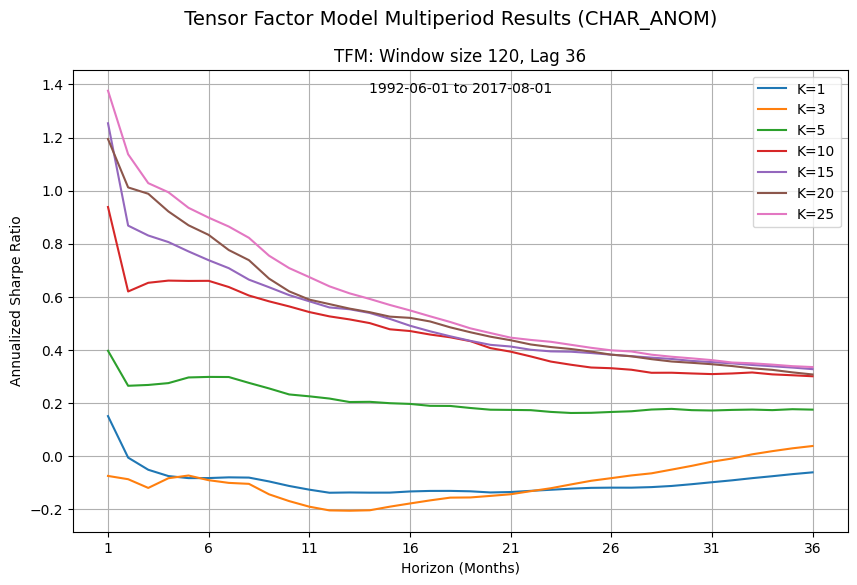
\includegraphics[width=1\linewidth]{full/char_anom_tensor_TFM.png}
    \caption{(CA) Tensor Factor Model: Full-Sample Sharpe Ratio}
    \label{fig:char_anom-primary-tfm}
\end{figure}

\begin{figure}[H]
    \centering
    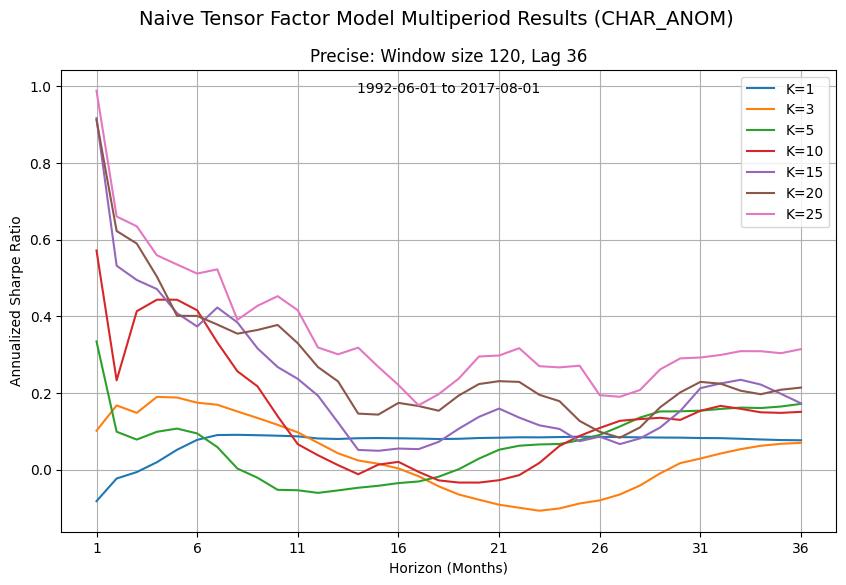
\includegraphics[width=1\linewidth]{full/char_anom_tensor_Precise.png}
    \caption{(CA) Precise Tensor Factor Model: Full-Sample Sharpe Ratio}
    \label{fig:char_anom-primary-precise}
\end{figure}

% \begin{figure}[H]
%     \centering
%     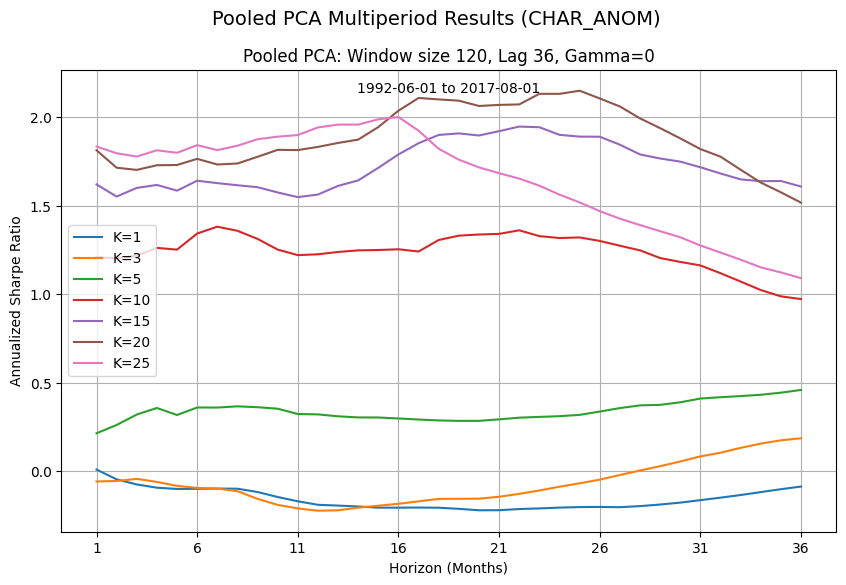
\includegraphics[width=1\linewidth]{full/char_anom_pooled_pca.png}
%     \caption{(CA) Pooled PCA Model: Full-Sample Sharpe Ratio}
%     \label{fig:char_anom-primary-pooled-pca}
% \end{figure}

\begin{figure}[H]
    \centering
    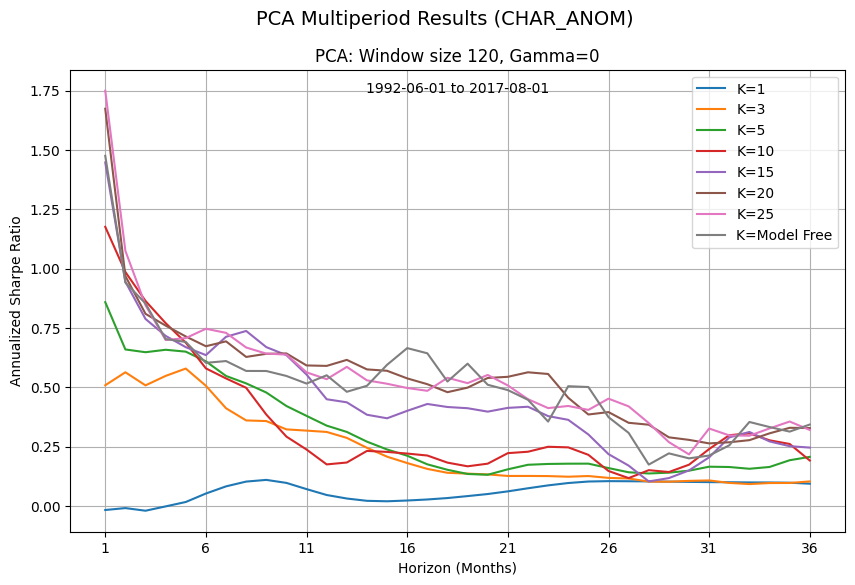
\includegraphics[width=1\linewidth]{full/char_anom_pca.png}
    \caption{(CA) Multiperiod PCA Model: Full-Sample Sharpe Ratio}
    \label{fig:char_anom-primary-pca}
\end{figure}


still need to add the pca graph for CA dataset + ensure that the model-free sharpes are included for all datasets


maybe a table that's like 

model $\implies$ K value (or model-free) $\implies$ sharpes for all 36 horizons

\subsubsection{Full-Sample SCS Dataset}

\begin{figure}[H]
    \centering
    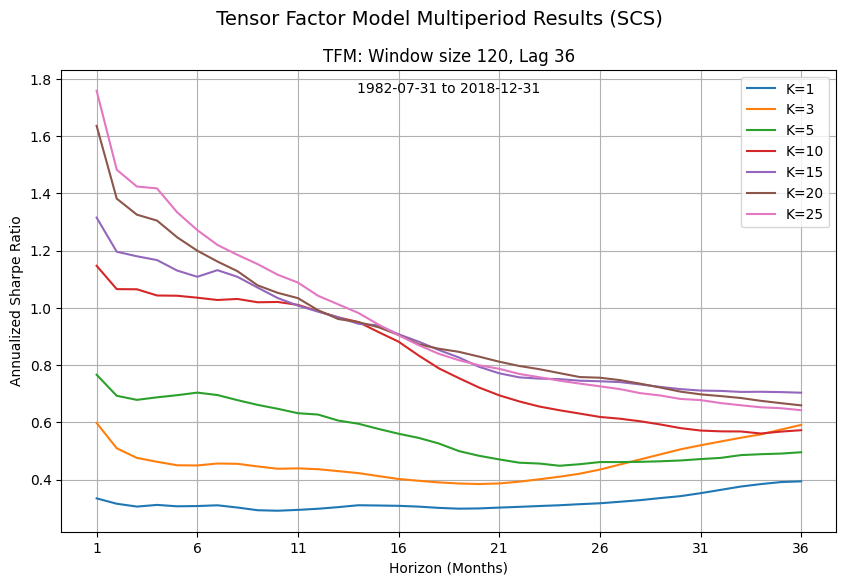
\includegraphics[width=1\linewidth]{full/scs_tensor_TFM.png}
    \caption{(SCS) Tensor Factor Model: Full-Sample Sharpe Ratio}
    \label{fig:scs-primary-tfm}
\end{figure}

\begin{figure}[H]
    \centering
    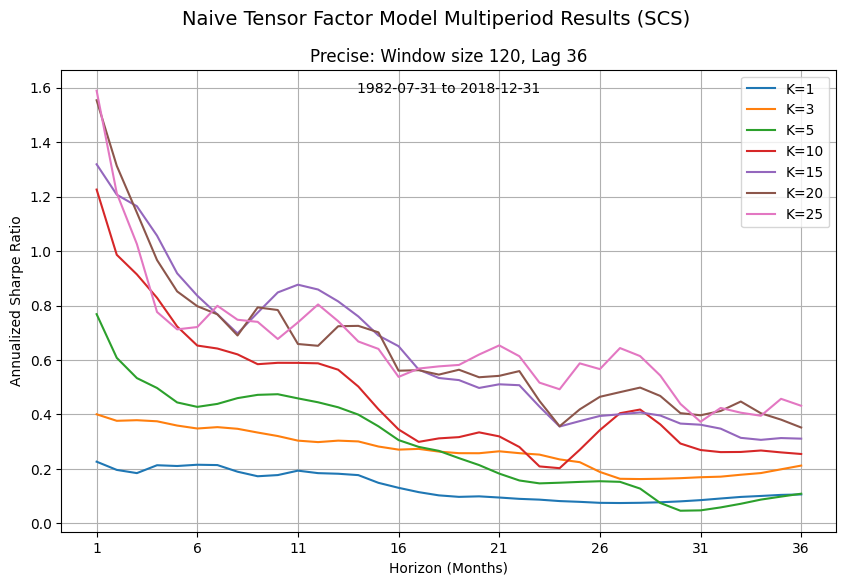
\includegraphics[width=1\linewidth]{full/scs_tensor_Precise.png}
    \caption{(SCS) Precise Tensor Factor Model: Full-Sample Sharpe Ratio}
    \label{fig:scs-primary-precise}
\end{figure}

% \begin{figure}[H]
%     \centering
%     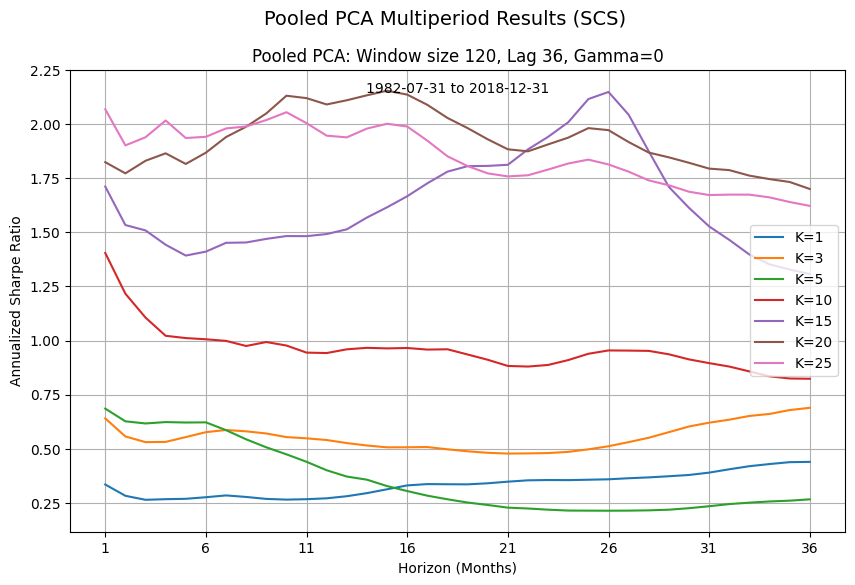
\includegraphics[width=1\linewidth]{full/scs_pooled_pca.png}
%     \caption{(SCS) Pooled PCA Model: Full-Sample Sharpe Ratio}
%     \label{fig:scs-primary-pooled-pca}
% \end{figure}

\begin{figure}[H]
    \centering
    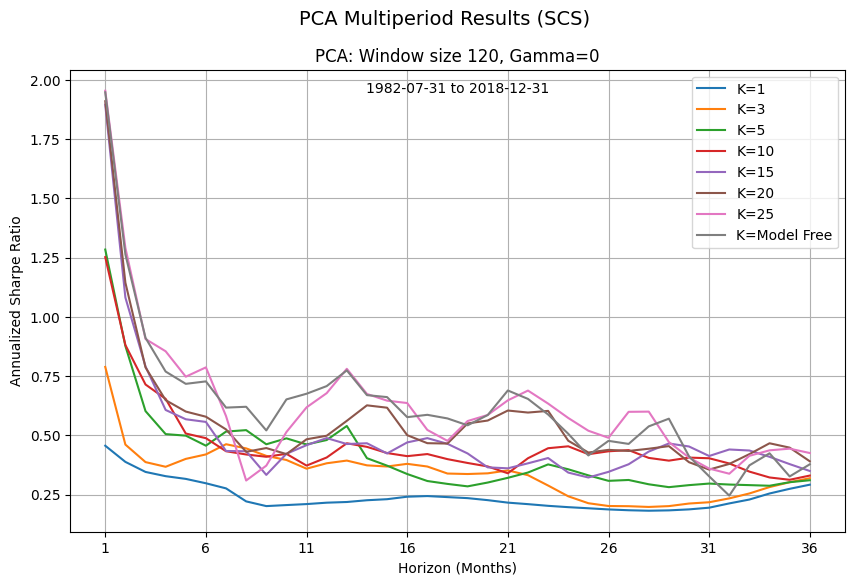
\includegraphics[width=1\linewidth]{full/scs_pca.png}
    \caption{(SCS) Multiperiod PCA Model: Full-Sample Sharpe Ratio}
    \label{fig:scs-primary-pca}
\end{figure}


\subsubsection{Full-Sample WRDS Dataset}

\begin{figure}[H]
    \centering
    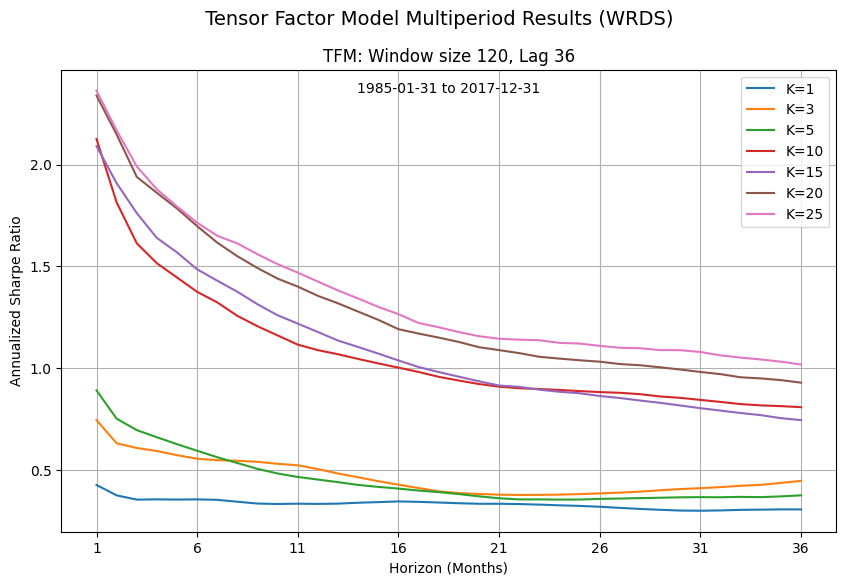
\includegraphics[width=1\linewidth]{full/wrds_tensor_TFM.png}
    \caption{(WRDS) Tensor Factor Model: Full-Sample Sharpe Ratio}
    \label{fig:wrds-primary-tfm}
\end{figure}

\begin{figure}[H]
    \centering
    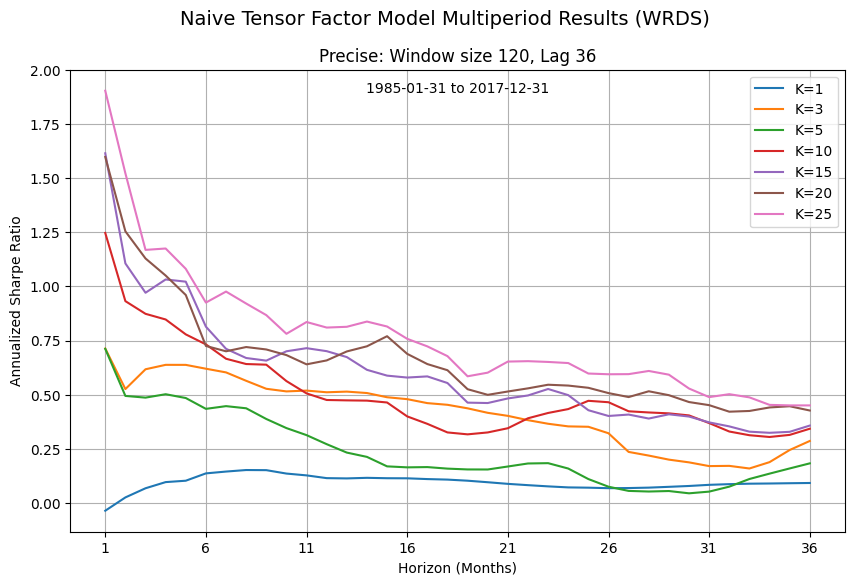
\includegraphics[width=1\linewidth]{full/wrds_tensor_Precise.png}
    \caption{(WRDS) Precise Tensor Factor Model: Full-Sample Sharpe Ratio}
    \label{fig:wrds-primary-precise}
\end{figure}

% \begin{figure}[H]
%     \centering
%     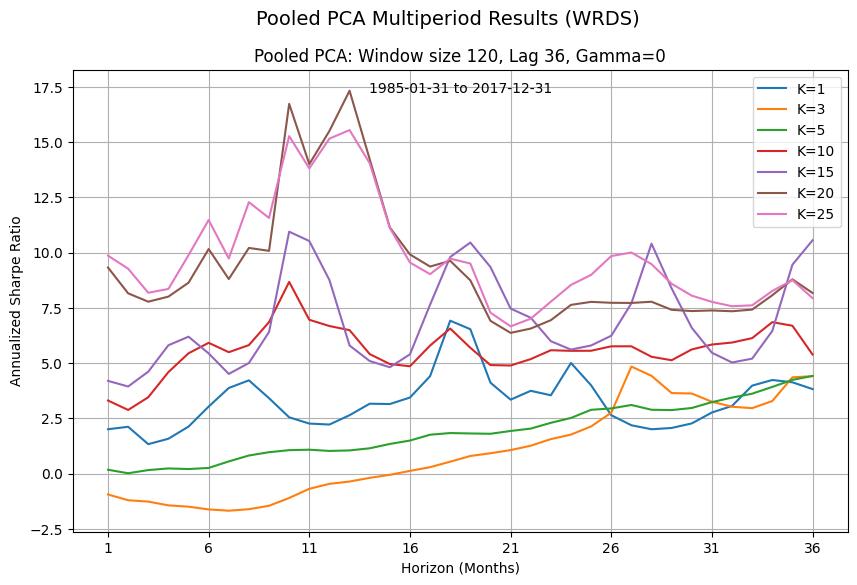
\includegraphics[width=1\linewidth]{full/wrds_pooled_pca.png}
%     \caption{(WRDS) Pooled PCA Model: Full-Sample Sharpe Ratio}
%     \label{fig:wrds-primary-pooled-pca}
% \end{figure}

\begin{figure}[H]
    \centering
    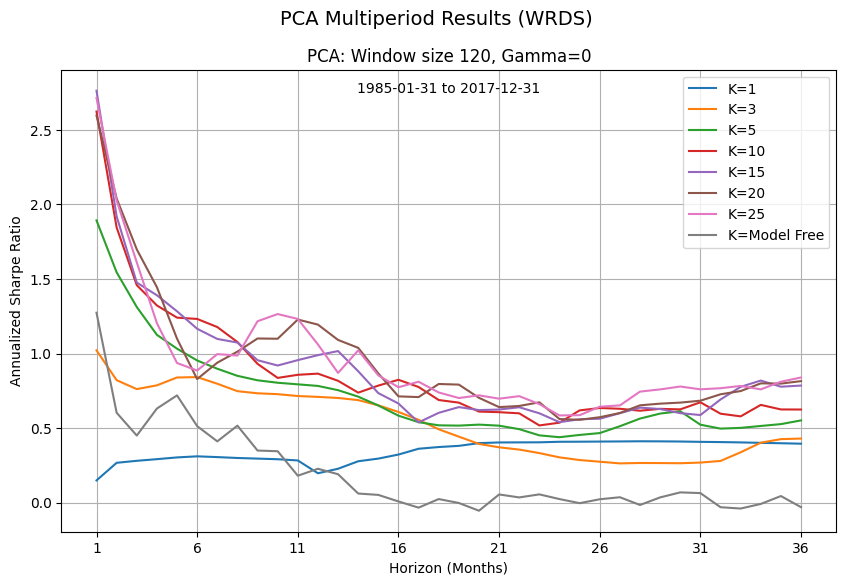
\includegraphics[width=1\linewidth]{full/wrds_pca.png}
    \caption{(WRDS) Multiperiod PCA Model: Full-Sample Sharpe Ratio}
    \label{fig:wrds-primary-pca}
\end{figure}


\newpage

\section{Appendix A}

\subsection{Primary Specification: OOS Results}

\subsubsection{OOS Characteristic Anomalies Dataset}

\begin{figure}[H]
    \centering
    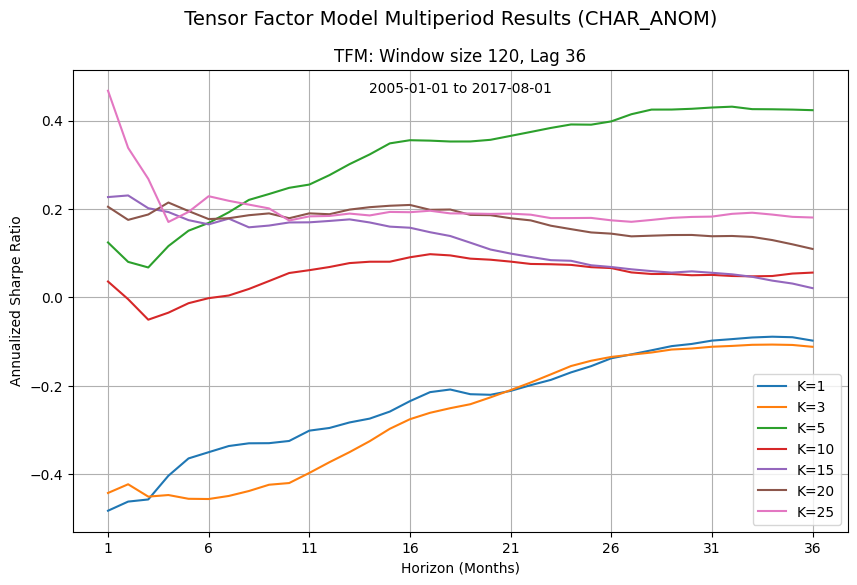
\includegraphics[width=1\linewidth]{oos/char_anom_tensor_TFM.png}
    \caption{(CA) Tensor Factor Model: OOS Annualized SR}
    \label{fig:char_anom-oos-tfm}
\end{figure}

\begin{figure}[H]
    \centering
    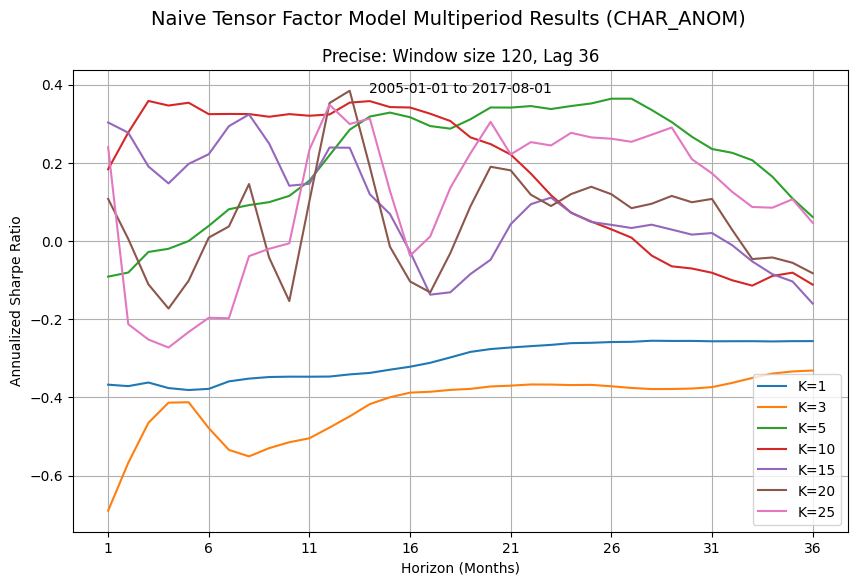
\includegraphics[width=1\linewidth]{oos/char_anom_tensor_Precise.png}
    \caption{(CA) Precise Tensor Factor Model: OOS Annualized SR}
    \label{fig:char_anom-oos-precise}
\end{figure}

% \begin{figure}[H]
%     \centering
%     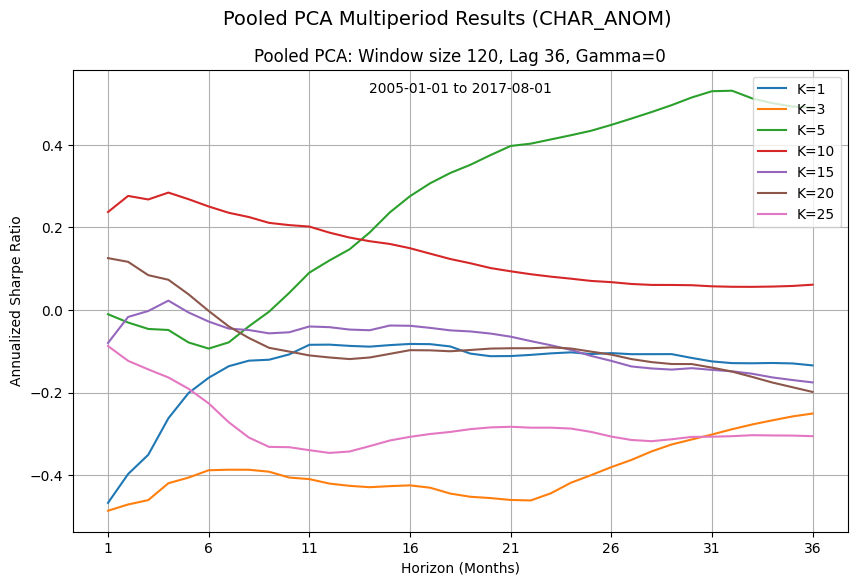
\includegraphics[width=1\linewidth]{oos/char_anom_pooled_pca.png}
%     \caption{(CA) Pooled PCA Model: OOS Annualized SR}
%     \label{fig:char_anom-oos-pooled-pca}
% \end{figure}

\begin{figure}[H]
    \centering
    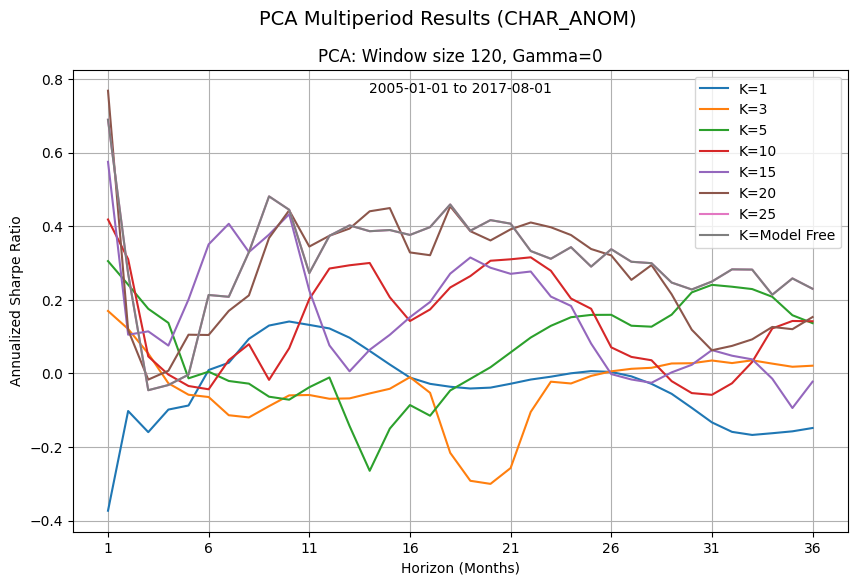
\includegraphics[width=1\linewidth]{oos/char_anom_pca.png}
    \caption{(CA) Multiperiod PCA Model: OOS Annualized SR}
    \label{fig:char_anom-oos-pca}
\end{figure}
    

\subsubsection{OOS SCS Dataset}

\begin{figure}[H]
    \centering
    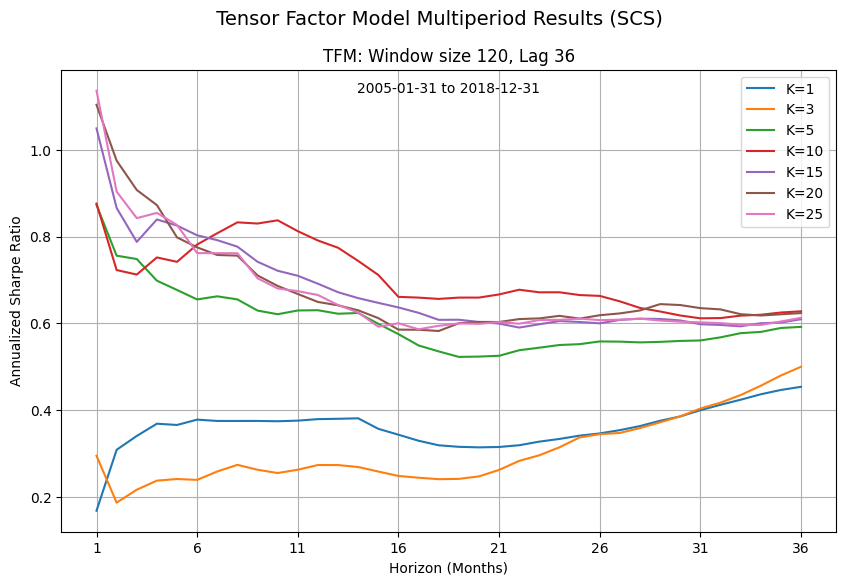
\includegraphics[width=1\linewidth]{oos/scs_tensor_TFM.png}
    \caption{(SCS) Tensor Factor Model: OOS Annualized SR}
    \label{fig:scs-oos-tfm}
\end{figure}

\begin{figure}[H]
    \centering
    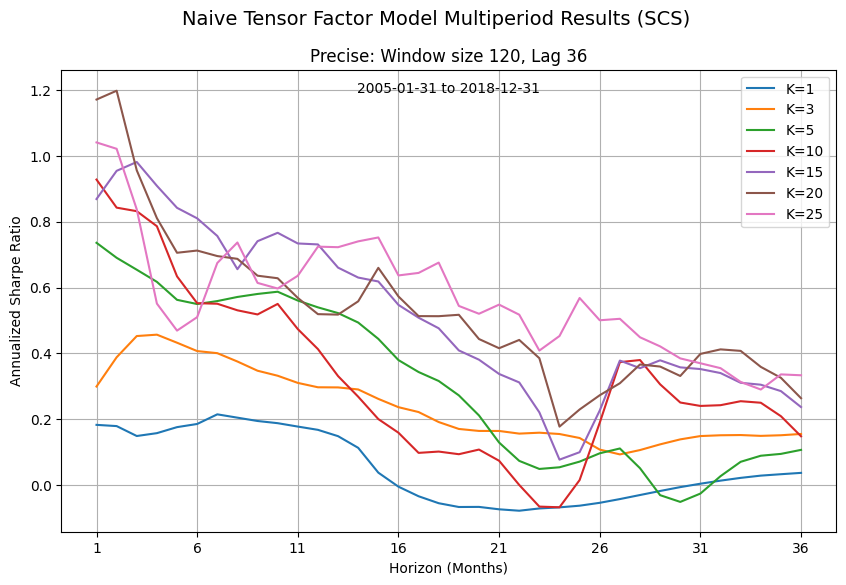
\includegraphics[width=1\linewidth]{oos/scs_tensor_Precise.png}
    \caption{(SCS) Precise Tensor Factor Model: OOS Annualized SR}
    \label{fig:scs-oos-precise}
\end{figure}

% \begin{figure}[H]
%     \centering
%     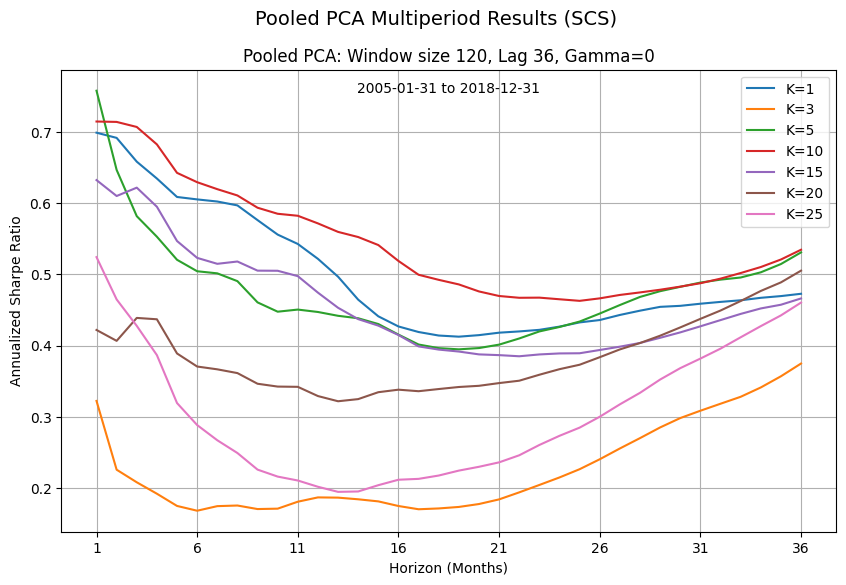
\includegraphics[width=1\linewidth]{oos/scs_pooled_pca.png}
%     \caption{(SCS) Pooled PCA Model: OOS Annualized SR}
%     \label{fig:scs-oos-pooled-pca}
% \end{figure}

\begin{figure}[H]
    \centering
    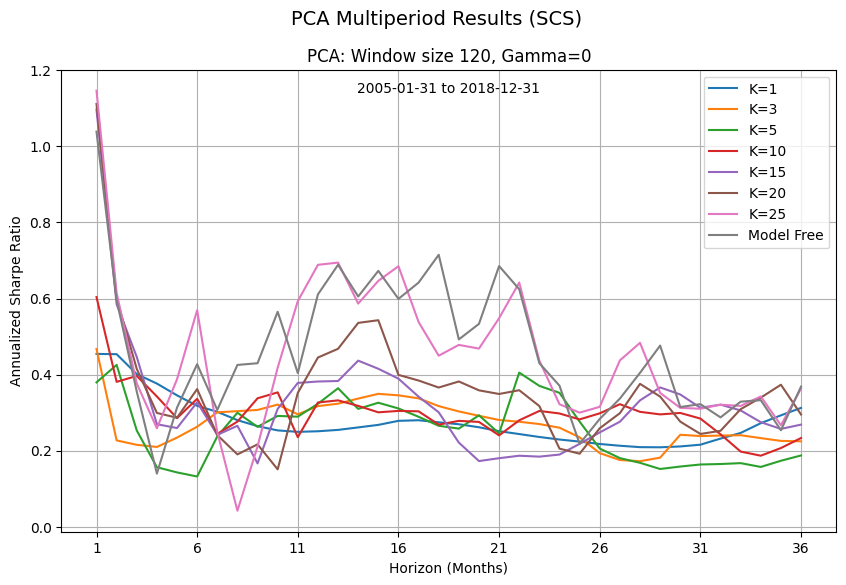
\includegraphics[width=1\linewidth]{oos/scs_pca.png}
    \caption{(SCS) Multiperiod PCA Model: OOS Annualized SR}
    \label{fig:scs-oos-pca}
\end{figure}


\subsubsection{OOS WRDS Dataset}

\begin{figure}[H]
    \centering
    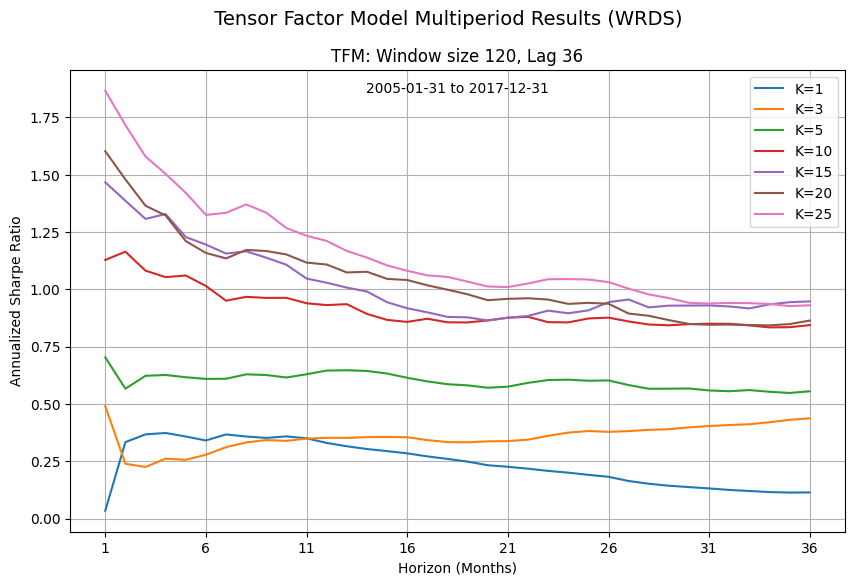
\includegraphics[width=1\linewidth]{oos/wrds_tensor_TFM.png}
    \caption{(WRDS) Tensor Factor Model: OOS Annualized SR}
    \label{fig:wrds-oos-tfm}
\end{figure}

\begin{figure}[H]
    \centering
    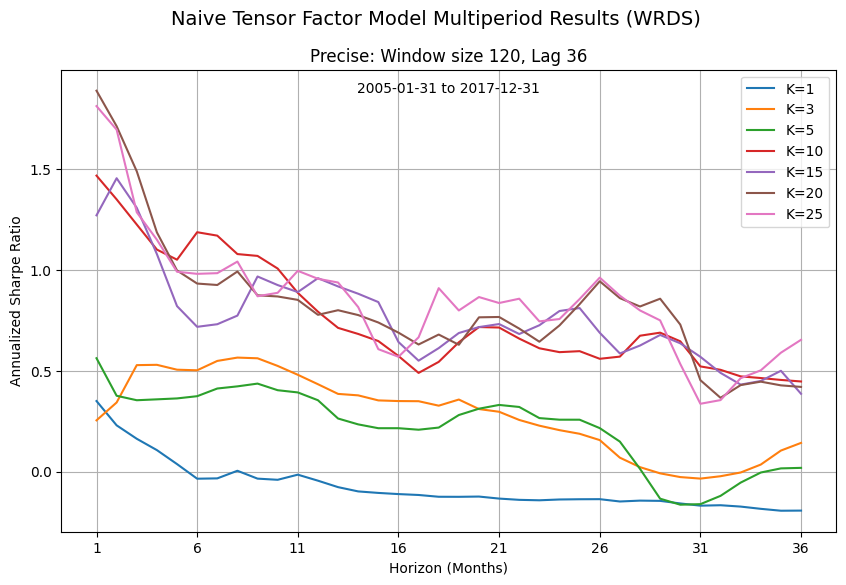
\includegraphics[width=1\linewidth]{oos/wrds_tensor_Precise.png}
    \caption{(WRDS) Precise Tensor Factor Model: OOS Annualized SR}
    \label{fig:wrds-oos-precise}
\end{figure}

% \begin{figure}[H]
%     \centering
%     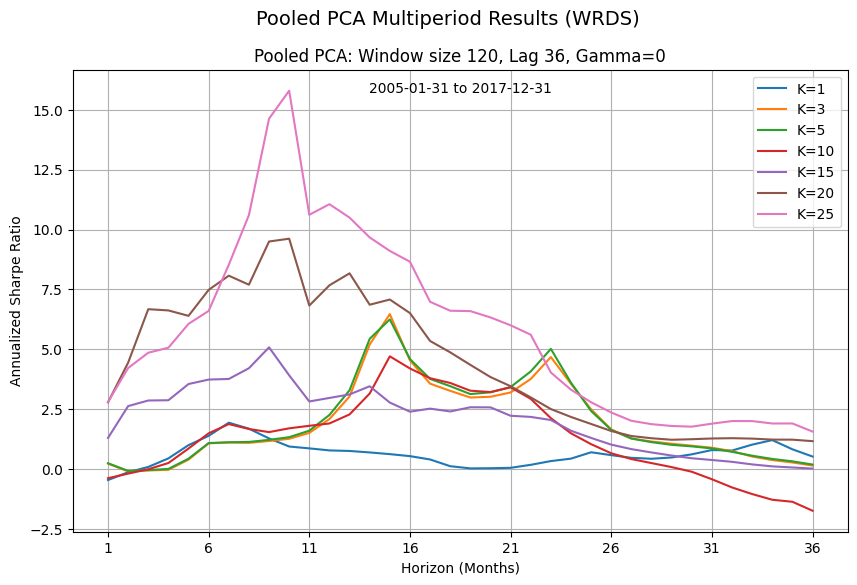
\includegraphics[width=1\linewidth]{oos/wrds_pooled_pca.png}
%     \caption{(WRDS) Pooled PCA Model: OOS Annualized SR}
%     \label{fig:wrds-oos-pooled-pca}
% \end{figure}

\begin{figure}[H]
    \centering
    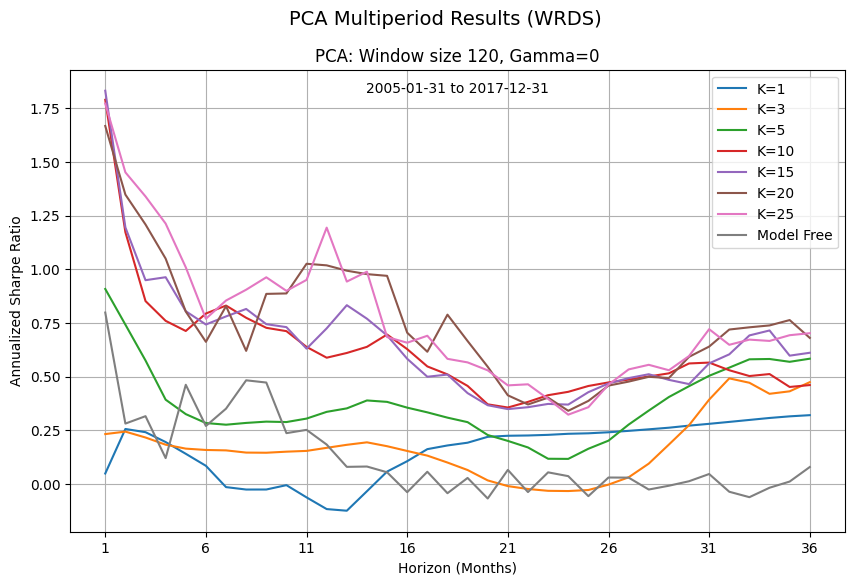
\includegraphics[width=1\linewidth]{oos/wrds_pca.png}
    \caption{(WRDS) Multiperiod PCA Model: OOS Annualized SR}
    \label{fig:wrds-oos-pca}
\end{figure}


% \section{Appendix B}

% \[\Lambda w_n = w_k \implies w_n = \Lambda_k^\dagger w_k\]
% \[w_n = \Lambda_k(\Lambda_k^T \Lambda_k)^{-1} w_k\]

\end{document}
